                                      %\\\\\\\\\\\\\\\\\\\\\\\\\\\\\\\\\\\\\\\\\\\\\\\\\\\\\\\\\\\\\\\\\\\\\\\\\\\\\\\\\\\\\\\\\\\\\\\\\\\\\\\\\\\\\\\\\\\\\\\\\\\\\\\\\\\\\\

%Preamble

\RequirePackage[l2tabu, orthodox]{nag}
\documentclass{article}
\usepackage[utf8]{inputenc}
\usepackage[usenames, dvipsnames]{xcolor}
\usepackage[english]{babel}
\usepackage[documents]{ragged2e}
\usepackage{comment}
% 9 LaTeX packages everyone should use
\usepackage{amsmath}
\usepackage[a4paper]{geometry}
\usepackage[rightcaption]{sidecap}
\usepackage[skip=true,justification=justified,singlelinecheck=false,font=small,format=plain,labelfont=bf,up,textfont=normal,up]{caption}
\usepackage{graphicx}
\graphicspath{ {DDfigures/} }
\usepackage{microtype}
\usepackage{siunitx}
\usepackage{booktabs}
\usepackage[
backend=biber,
style=authoryear,
sorting=ynt
]{biblatex}
\addbibresource{DD_for_energy_management.bib}
\usepackage{gensymb}
\usepackage{csquotes}
\usepackage{hyperref}
\hypersetup{
    colorlinks=true,
    linkcolor=blue,
    filecolor=magenta,      
    urlcolor=cyan,
}
\urlstyle{same}
\usepackage{cleveref}

%\\\\\\\\\\\\\\\\\\\\\\\\\\\\\\\\\\\\\\\\\\\\\\\\\\\\\\\\\\\\\\\\\\\\\\\\\\\\\\\\\\\\\\\\\\\\\\\\\\\\\\\\\\\\\\\\\\\\\\\\\\\\\\\\\\\\\\

\begin{document}

% Title stuff
\title{Use of Degree Days in Energy Management}
\author{Michael Hunt}
\date{\today}
\maketitle

%\\\\\\\\\\\\\\\\\\\\\\\\\\\\\\\\\\\\\\\\\\\\\\\\\\\\\\\\\\\\\\\\\\\\\\\\\\\\\\\\\\\\\\\\\\\\\\\\\\\\\\\\\\\\\\\\\\\\\\\\\\\\\\\\\\\\\\

\section{Introduction}

For these lectures we will use gas heating and hot water data taken from my house over a three period. The meter is an old fashioned one of the type that we mostly all still have in our houses, where the readings have to be taken manually. In commercial settings these meters have been superseded by "smart" meters by which we mean that they automatically log and store readings at least once every half hour. In time, these will become the norm in domestic settings, but for the moment, a meter like mine is all we have to go on.
The purpose of the exercise here is to see what can be gleaned from the limited information that this meter provides about how the energy usage of the house is split between space heating and hot water, how well the control systems work and whether there is a fault.\\


We will learn :

\begin{itemize}
  \item How to interpret the meter readings, given in m$^3$ and convert them to kWh.
  \item How to interpolate between meter readings taken on given dates to find estimated readings for the beginning of each month.
  \item To understand the meaning and usage of the concepts of degree days and base temperature and where to find current and historical values for a range of locations.
  \item How to determine the base temperature of the house.
  \item How to construct and interpret a performance line for monthly degree day data.
  \item How to disaggregate the separate energy usages for space heating and hot water given a single gas meter.
  \item How to conduct and interpret a CUSUM (Cumulative Sum of Errors) analysis of the data.
  \item How to use the data as an aid to strategies for action - does anything need fixing? What needs doing?
\end{itemize}

The lectures closely follow the methodology given in the Carbon Trust document Degree Days for Energy Management \cite{CarbonTrust2012}.\\

\section{Spreadsheet remarks}


This year (2014-2015) we will carry out the analysis required for this exercise in Excel. However it is worth noting that this is not the only possibility, and that we could, for example, also carry it out in Google Sheets. For our day to day purposes these two different spreadsheet applications work almost identically. Virtually all the formulae that are used in Excel work in the same way in Google Sheets so if you are familiar with one you will very quickly be able to work in the other. Of course, some things are different - there would be no sport if that were not true \textit{some} of the time - and we will highlight where that occurs below. But if you can use one, you will be able to use the other.\\

As part of the Microsoft Office suite, Excel is (2014, watch this space!) the de facto world standard spreadsheet application and is a fancier, altogether flashier looking beast than Google Sheets. However, the digital world changes rapidly and I am deliberately exposing you to Google Sheets so that you do not go through this course without realising that there is more than one spreadsheet application out there.\\

Google Sheets has some advantages over Excel. It is free, for one thing! It looks simpler, because it is, yet it is for most peoples' purposes, most of the time, perfectly good enough, and in that case, whatever is simplest (and free!) could well be the best. Moreover, Google Sheets is saved "in the Cloud", so anything done anywhere is accessible from anywhere that has an internet connection. I have found this to be a huge advantage when juggling between work/college and home. It immediately solves the problem of having different versions of your work in different places, and often enough, in the wrong place. You can also "share" your files with others, such as your tutor, or your peers. I do this a lot, as you will have noticed, but so do others. The Guardian newspaper, for example, often shares the data behind a news story in a Google Sheets spreadsheet.\\
\begin{comment}{
\subsection{Differences between Google Sheets and Excel}
\begin{enumerate}
\item \textbf{Dynamic ranges} aren't quite so conveniently achieved in Google Sheets as they are in Excel. 
\item User defined functions are written in \textbf{VBA} in Excel and in \textbf{JavaScript} in Google Sheets. In this module we use one user defined function interpdate
\end{enumerate}
}
\end{comment}

When the analysis is complete, we will compare the way we did it in Excel with how we could have done it in Google sheets, to illustrate the similarities and differences between the two applications.\\

Right, let's go.......\\

Open the template file "\textbf{Degree Days for Energy management template}".\\

A link to this given on the Moodle site for the module. Make your own copy of it and use this from now on.\\

\section{Converting the meter readings to kWh}
The first problem is that we are interested in energy usage, yet the gas meter actually records the \textit{volume} of gas that has passed through it. This needs to be converted to an energy. To do this we need to know the energy density (energy per unit volume) of the natural gas supplied to the house.
\begin{enumerate}
\item On the "\textbf{Data}" Sheet there are gas meter readings for my house over a period of several years. The meter was mostly read on Saturday mornings, but there are a few gaps, for example, for holidays. The meter reading gives volume of gas supplied in m$^3$. We need to convert this to energy supplied in kWh.\\
To do this we need to know the energy density of the natural gas supplied to the house, in kWh m$^{-3}$ This value is found by multiplying a value provided by the supplier that is correct for the content of the gas (which may change with time) and for a specified set of temperature and pressure conditions, by a density correction factor to allow for the (supposed) actual conditions. Both these values are normally given on the bill from the supplier. The energy density is about 39.2 kWh m$^{-3}$ under standard conditionms, and the correction factor is given as 1.02264.
\item In column F, generate values for the energy supplied in kWh ie what the meter would read if it read in kWh rather than m$^3$. 
\item We will need to refer to the ranges that contain the dates and the supplied energy values we have just calculated, and it will be handy if we name these ranges and, especially, if we do so \emph{dynamically}. This means, do so in such a way that the ranges will grow when we add more data, as we take more readings. This is a common problem. Dynamic naming of ranges that are likely to grow, as here, is very useful. In Excel, you can do this using the {\color{blue}OFFSET} command in Formulas/Name Manager.
Use the names \emph{date} and \emph{meter\_kWh} for the two ranges. In the box where you specify the cells to which you are giving a name you write a formula with the {\color{blue}OFFSET} command in which (this is the cunning bit) the {\color{blue}COUNT} command is embedded .For the \emph{date} name, for example, the command will look like this:
{\color{blue}
\begin{verbatim}
 =OFFSET(Data!$A$4,0,0,COUNT(Data!$A:$A),1)
 \end{verbatim}
}
aswe see in Figure \ref{fig:dynamicrange}.
\begin{SCfigure}[0.5][ht]
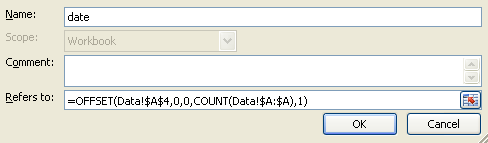
\includegraphics[width=0.6\textwidth]{dynamicrange}
\caption{Use of the {\color{blue}OFFSET} and {\color{blue}COUNT} commands to create a dynamic range}
\label{fig:dynamicrange}
\end{SCfigure}
This command specifies a block of cells that starts at {\color{blue}{\$A\$4}}, has as many rows as there are rows containing numbers in column A (that is what {\color{blue}COUNT(Data!\$A:\$A)} tells us), and is 1 column wide.
\end{enumerate}
\section{Monthly energy usage}
We now wish from this list of meter readings in kWh to find how the energy used in each month depends on the severity of the weather in that month.
\begin{enumerate}
\item On the "Energy per Month" Sheet, beneath the titles rows provided, set up in column B a series of dates, each one the first of the month,  starting 01/09/2008/. Continue this series to 01/02/2012. Reformat this series to that it appears as Sep-08, Oct-08 etc. You can do this in Home/Number/Custom/mmm-yy
\item In column C, enter monthly degree day data for Camborne, with a Base Temperature of 15.5\degree. This is a commonly used base temperature, but it may not be correct for my house. We will investigate that shortly. The data are to be found on the \href{http://www.eci.ox.ac.uk/research/energy/degreedays.php}{ECI site} \cite{ECIOxfordUniversity2014} - scroll to the bottom and download the csv file of month heating degree data for Camborne.
\item If you wish to find out more about degree days, see some notes I have written , displayed on the Moodle site for this module, or the Carbon Trust's helpful guide Degree days for Energy Management \cite{CarbonTrust2012}.
\item In column D, use the \textbf{interpolate\_1D} user-defined function to estimate what the meter reading would have been, in kWh, at the beginning of each month. This is an important and commonly required step, since the actual meter readings are taken according a regular(ish) weekly schedule (every Saturday) that means that readings are not normally taken on the first day of each month
\item In column E, calculate the energy content of the gas, in kWh, used each month by the house. The value for Oct-08 will be the meter reading in kWh on 1st Oct 2008 minus the reading on 1st September 2008, and so on.
item The sheet should now look something like Figure \ref{fig:EPMsheet}:

\begin{SCfigure}[0.5][ht]
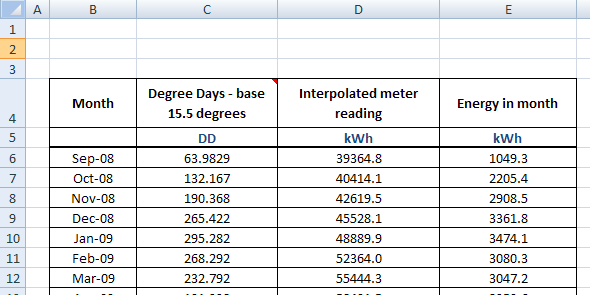
\includegraphics[width=0.6\textwidth]{SEM_L1_im_001}
\caption{The Data sheet after use of interpolation to estimate meter readings at the beginning of each month readings to kWh, and calculation of monthly energy usage}
\label{fig:EPMsheet}
\end{SCfigure}

\item On the same sheet, plot a scatter plot of Energy usage / month vs month.
\textit{
\begin{itemize}
\item Can you tell at what times of year the heating is turned on and off in this house?
\item Can you estimate from this chart how much energy is used per month for hot water and cooking? 
\end{itemize}
}
\end{enumerate}
\section{The Performance Line and what it tells us}

It is easy to perceive the seasonal cycles from the data when plotted as above, but it is difficult to meaningfully compare the energy usage of one period with another because many factors are at work: one year may be milder than another and so affect energy usage, but changes to the fabric or number of occupants of the house may also change energy usage too. \\It is easier to disentangle these factors if instead, monthly energy data are plotted against degree days per month. That is what we will do  in this section. 
\begin{enumerate}
\item Use the {\color{blue}OFFSET} command to name dynamic ranges for the Months, Degree days per Month and kWh per Month. Use the names \emph{months}, \emph{kWh\_Monthly} and \emph{DD\_monthly}. You need to write this command into the Name Manager.For the \emph{months} name, for example, the command will look like this:

{\color{blue}
\begin{verbatim}
 =OFFSET('Energy per month'!$B$6,0,0,COUNT('Energy per month'!$C:$C),1)
 \end{verbatim}
}
\item Plot a scatter plot of Energy in Month against Degree days per month. Add a linear trend line (Excels way of describing a line of best-fit by linear regression), find the slope and gradient of this and the Pearson R2 correlation coefficient. You should get something like Figure \ref{fig:perf_line_at_BT_15.5}:

\begin{SCfigure}[0.5][ht]
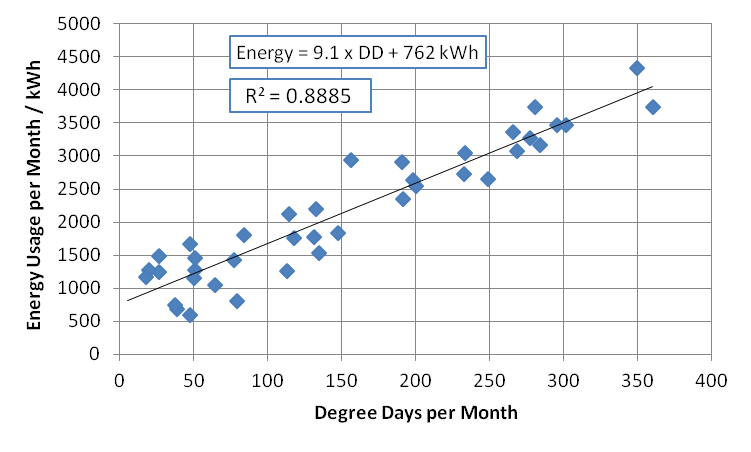
\includegraphics[width=0.6\textwidth]{Monthly_Energy_vs_DD_15_5_BT}
\caption{Monthly gas energy usage vs degree days per month, using a base temperature of 15.5$\degree$. A best fit straight line has been added. This is called the performance line.}
\label{fig:perf_line_at_BT_15.5}
\end{SCfigure}
{\color{OliveGreen}
\begin{itemize}
\item Notice that the more degree days there are in a month, the more energy tends to be used. There is some scatter but a linear correlation between the energy usage and degree days for a month seems evident, so it is reasonable to fit a straight line to the data. We cannot tell which point on the plot occurred when, just that those in the top right are from cold months and those in the bottom left are from warmer months. 

\item The straight line fit is called a \textbf{Performance Line} for the building and the equation for it can be used to predict energy usage in this building in any month, given the degree days for that month. 

\item \textit{What do the \textbf{gradient} and \textbf{intercept} of this plot tell us?} \\The gradient (9.1 kWh per DD here) tells us how many extra kWh per month are used for every extra degree day in that month. It is therefore driven by temperature differences and is an indication of the space heating requirement of the building. The intercept (762 kWh here) is positive, which means that there is energy usage even when there are no degree days for the month. This energy usage cannot therefore be driven by temperature difference, and must be the cooking (but there is only a gas hob) and (mainly) hot water usage of the house. According to this performance line, this house uses 762 kWh per month, or about 25 kWh per day for hot water usage. Is this reasonable or not for this house? Answering that may take some further thought, but at least now we have an idea as to how many kWh per month are used for hot water and not for space heating.

\item The \textbf{Pearson R2 correlation factor} is an indicator of how well the line fits the data. R2 always lies between -1 and 1. For positively correlated data, as we have here (line of best fit has positive gradient) R2 is always between 0 and 1, and where there is a good fit, R2 is greater than about 0.8. Where there is a perfect fit, R2 = 1. The better the fit, the less the scatter. We have included the R2 value because, while we have a performance line, we don't know yet whether we have chosen the correct baseline temperature for this house. If we have not, the predictions of the performance line may be false.\\ We turn now to how to determine the actual base line temperature for this house: it will be that temperature which gives the best fit to a regression in a performance line plot ie for which the R2 value of the performance line is greatest.

Apart from helping us select the actual base temperature, the  R2  value is an indication of the effectiveness of the heating control systems in a building. A low value of  R2  means that the building energy use does not closely follow the weather, perhaps because of a faulty thermostat or an under sized heating system. Poor control systems lead to higher costs since more heat is wasted.
\end{itemize}
}
\end{enumerate}

\section{Establishing the correct base-temperature} 
The base temperature of 15.5$\degree$, though widely used, is not necessarily correct for this house. It is important to get it right, since a degree day analysis of space heating energy data will make wrong predictions if the wrong base temperature is used.\\

On the "\textbf{Find the Base Temperature}" Sheet, 
\begin{enumerate}
\item In Columns B, Q and R, under the title headings, paste in the Month, Interpolated Meter Reading (kWh) and Energy in Month data from the "Energy per Month" sheet.
\item From the \href{http://www.eci.ox.ac.uk/research/energy/degreedays.php}{ECI site} site, find degree day data for Camborne for all base temperatures from 11 ºC  to 17.5 ºC and paste them into the columns below the title headings, between columns C and P.
\item Now for the neat bit. Instead of plotting a performance line for each base temperature, we can use the {\color{blue}RSQ} command of Excel to find it for us, without having to plot anything. We enter this command in the cells in the row labelled {\color{blue}RSQ}. We enter (if the Sep-08 data is in row 8)
{\color{blue}
\begin{verbatim}
 = RSQ(ydata,xdata) 
 \end{verbatim}
 }
 so here, for example for the 11 ºC base temperature, we write
 {\color{blue}
 \begin{verbatim}
 = RSQ(kWh_monthly,$C$10:$C$48)
\end{verbatim}
}
\item Scan along the line of R2 values and identify the one which is highest. If you like, use the {\color{blue}RANK} command in line 4 (or wherever you have put it) and find the base temperature that has RANK 1 (top!).\\
\begin{itemize}
\item \textit{Which base temperature does this correspond to? [Ans: 14 ºC]}
\end{itemize}
\item Plot R2 vs base temperature. You should get something like Figure \ref{fig:r2_vs_BT_plot}

\begin{SCfigure}[0.5][ht]
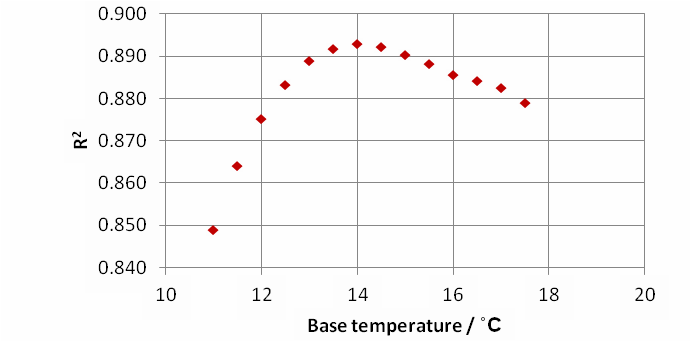
\includegraphics[width=0.6\textwidth]{r2_vs_BT_plot}
\caption{A plot of the Pearson r$^2$ parameter for performance lines fitted to plots of monthly energy usage against degree days for the month, as a function of base temperature. The higher the value of r$^2$, the better the fit of the performance line to the data, implying a better choice of base temperature.}
\label{fig:r2_vs_BT_plot}
\end{SCfigure}

\begin{itemize}
\item \textit{From this graph, can you tell if one base temperature is clearly more suitable than the others? Which one? [14 ºC]}
\end{itemize}

\item Similarly, we can find the gradient and intercept of the performance line for all these base temperatures without having to plot the graph. We use the commands {\color{blue}SLOPE} (ydata,xdata) and {\color{blue}INTERCEPT} (ydata, xdata) which work in the same way as the {\color{blue}RSQ} command. Again for ydata we use the named range kWh\_monthly, and for xdata we use the monthly degree days for each temperature. For example,
{\color{blue}
\begin{verbatim}
 = SLOPE(kWh_monthly,$C$10:$C$48) 
 = INTERCEPT(kWh_monthly,$C$10:$C$48) 
\end{verbatim}
}
give the gradient and intercept respectively of the performance line drawn for degree day data of the base temperature in column C. Your sheet should now look something like Figure \ref{fig:SlopeIntercept}, with the energy data over in columns Q and R, to the right of all the degree day data:

\begin{SCfigure}[0.5][ht]
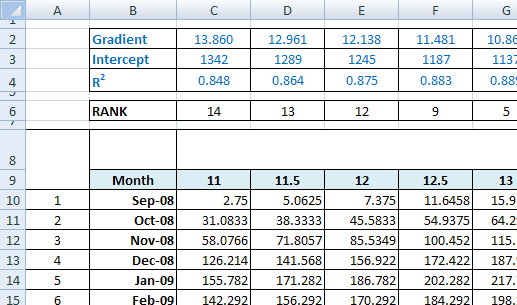
\includegraphics[width=0.6\textwidth]{SEM_L1_im_003}
\caption{Use of the {\color{blue}SLOPE} and {\color{blue}INTERCEPT} commands to find the gradient and intercept of several performance lines}
\label{fig:SlopeIntercept}
\end{SCfigure}

\begin{itemize}
\item \textit{Do the predicted monthly usages of energy for hot water and cooking differ when different base temperatures are used?}
\end{itemize}

Yes they do - the intercept values in the performance plot are different for each base temperature. Either they are all wrong or... the truth is that degree days are a bit crude as a concept, so our take on this is that  predictions using one particular base temperature are more likely to be right any made using the others - the one for which the performance line gives the best fit to the data. 
\end{enumerate}

\section{On the Monthly Analysis sheet:}
\begin{enumerate}
\item Fill in the columns A to D under the titles, where for the degree day data in column B you use that set for the correct base temperature.
\item Dynamically name the range containing the degree day data, using the {\color{blue}OFFSET} command. Call it DD\_BF\_monthly.
{\color{blue}
\begin{verbatim}
 = OFFSET('Monthly Analysis'!$B$8,0,0,COUNT(kWh_monthly),1)
\end{verbatim}
}
\item Plot a performance line plot : Energy in Month vs Monthly Degree days.
\item Add the performance line using (what Excel calls) the linear Trend line.
\item In three cells near the chart, find and clearly display the gradient, intercept and R2 values for the performance line. You should get something like Figure \ref{fig:best_fit_pf}

\begin{SCfigure}[0.5][ht]
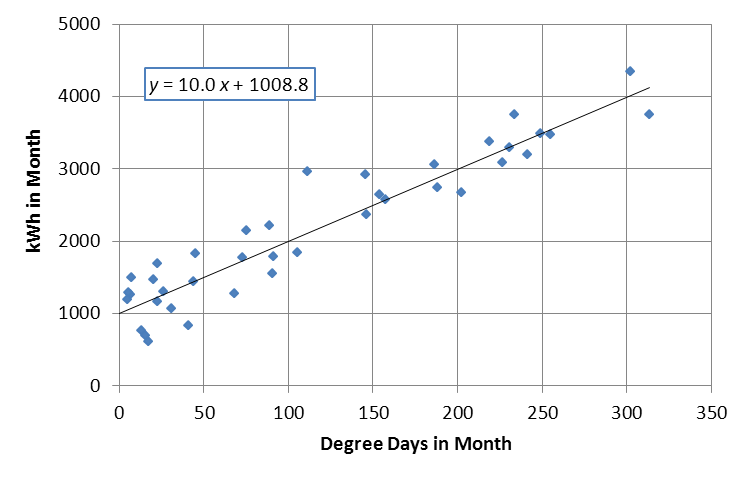
\includegraphics[width=0.6\textwidth]{optimal_performance_line}
\caption{The performance line for the building drawn using the optimal base temperature of 14 $\degree$. The line has a slope of 10.0 kWh per DD, and an intercept of 1009 kWh per month}
\label{fig:best_fit_pf}
\end{SCfigure}
\end{enumerate}

\begin{itemize}
\item \textit{How much energy does this household use per month for hot water and cooking, do you now think?}[Ans: 1009 kWh - the intercept of the performance line, since this is the energy usage at zero $DD$]

\item \textit{How much energy does this household use per year for hot water and cooking, do you now think?}[Ans: $12 \times 1009=12108$ kWh - twelve times the intercept of the performance line, since this is the energy usage per month at zero $DD$]

\item \textit{How much additional energy would this household use for every extra degree day?}[Ans: 10.0 kWh, since this is the gradient of the performance line. The units of the gradient are kWh per $DD$ - so the gradient is the additional energy usage per every extra degree day]

\item \textit{In a month where there are 200 degree days, how many kWh of gas does the performance line predict that this household would use in total?}[Ans: $1009 + 10.0 \times 200 =\ about\ 3009$ kWh]

\item \textit{If the gas costs 4p per kWH, how much does the performance line predict that the gas would cost for a month with 150 degree days?}[Ans: $0.04 \times (1009 + 10.0 \times 150) =  \pounds 100$]
\end{itemize}

\section{Troubleshooting - is everything working as it should?}
So now we have a tool that (we hope) helps us determine how much gas this building will use in future. Now, let's be Good Energy Managers and master a tool that will help us determine if the building is working as it is supposed to. To do this we will carry out a a CUSUM (Cumulative Sum Of Errors) analysis.\\
On the \textbf{Monthly Analysis sheet},
\begin{enumerate}
\item In the Performance Line Energy column, we need to calculate the energy predicted for each month by the performance line. This can be done in a number of ways in Excel, but the easiest is to use the {\color{blue}FORECAST}(x, known\_y's, known\_x's) command.  This calculates a new y-value for a given x-value given a set of values of x and y, assuming a straight line fit. Here the, x-values are the degree days per month (DD\_BF\_monthly) and the y-values are in the range containing the monthly energy usage values, which we have named KWh\_monthly, so
{\color{blue}
\begin{verbatim}
 = FORECAST(B8,kWh_monthly,DD_BF_monthly)
 \end{verbatim}
}
would give the performance line value for the energy usage in Sep-08, if that month is in row 8.

Using the {\color{blue}FORECAST} command, fill in the performance line predictions for energy usage for every month in our data.

\item In the Delta column, find the error between actual and predicted energy usages in each month, where the error is defined as actual usage - predicted usage.
\item In the CUSUM column, in each row calculate the cumulative sum of the errors up to that row. The cumulative sum up to Dec-08, 671.9 kWh is calculated using {\color{blue}\begin{verbatim}=SUM($F$8:F11)\end{verbatim}}, for example

Your sheet should now look something like Figure \ref{fig:forecast_command}

\begin{SCfigure}[0.5][ht]
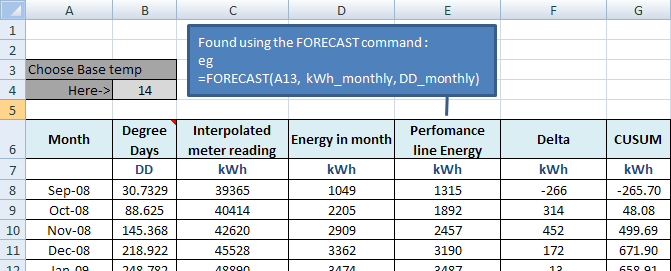
\includegraphics[width=0.6\textwidth]{forecast_command}
\caption{Use of the {\color{blue}FORECAST} command to calculate the predicted energy usage for each month, based on the performance line of \textbf{Figure} \ref{fig:best_fit_pf}}
\label{fig:forecast_command}
\end{SCfigure}

\item \textbf{Interpretation of CUSUM plot}: Now plot the cumulative errors against month as in Figure \ref{fig:CUSUM_plot}:

\begin{SCfigure}[0.5][ht]
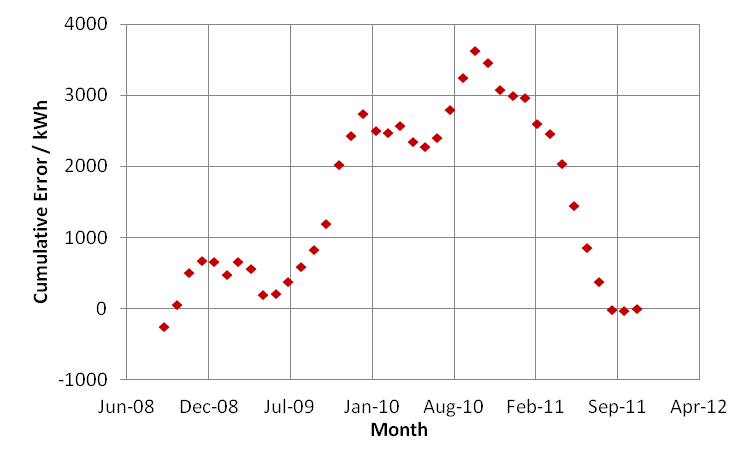
\includegraphics[width=0.6\textwidth]{CUSUM_plot}
\caption{CUSUM plot for the property - where the CUSUM is rising, the building's performance is getting worse, and where it is falling, it is improving}
\label{fig:CUSUM_plot}
\end{SCfigure}

{\color{OliveGreen}This plot alerts us to possible changes in the thermal performance of the building. If the CUSUM value is rising, the performance is getting steadily worse, and if falling, it is getting steadily better. In our data, we see a steady(ish) rise until October 2010 and then a steep fall. This is the power of a CUSUM analysis: it is an indicator of change. We can see from this plot that the energy usage of the property was getting steadily worse, against historical patterns, up to October 2010. If this plot had been started and kept going from September 2008 it would, at least by September 2009, have indicated that something was happening that needed investigating. 
}

\item What was going on before October 2010, and what happened then to reverse this trend?
\\To help answer this, plot separate performance lines for data up to October 2010 and for data after October 2010. You should get something like Figure \ref{fig:PrePost_Performance_Lines}:

\begin{SCfigure}[0.5][ht]
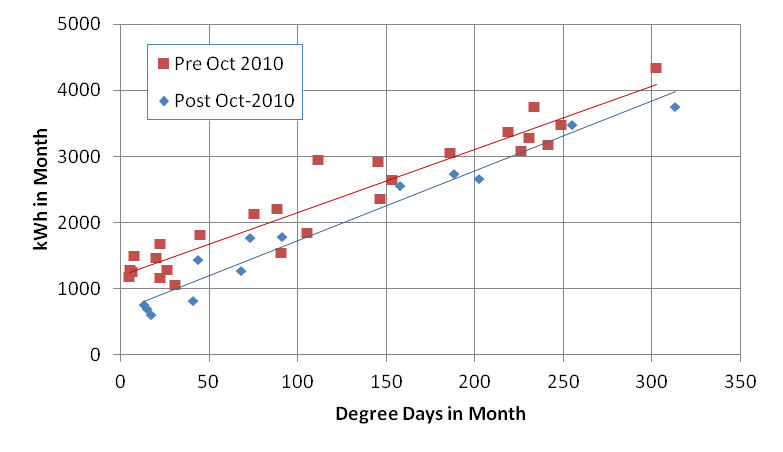
\includegraphics[width=0.6\textwidth]{PrePost_Performance_Lines}
\caption{Two performance lines drawn for the same property, one for data before October 2010, one for data after that date.}
\label{fig:PrePost_Performance_Lines}
\end{SCfigure}

After October 2010:
{\color{OliveGreen}
\begin{itemize}
\item \textit{Was the space heating energy demand significantly changed?} \\\textbf{No}, the slopes of the two performance lines are very similar
\item \textit{Was the hot water energy demand significantly changed?} \\ \textbf{Yes}, the intercept of the performance line after October 2010 is much less than before

\item \textit{What do you think happened at the property in October 2010?} \\ \textbf{Either} there was a sudden change in the behaviour of the occupants, for example a switch from baths to showers, or a decision to take shallower baths, or to change the shower head, \textbf{or} the number of occupants suddenly fell, \textbf{or} the settings on the hot water heating controls were altered, or..... 
\\In fact that is what happened - the hot water had been on a continuous setting because a valve was faulty and would not reopen if an intermittent setting was used. In October 2010 the valve was replaced, an intermittent setting was used thereafter and  the energy demand for hot water fell by 530 kWh per month, representing a monthly saving of about £20. A timely  CUSUM plot could have identified and quantified the problem at least a year before it was addressed, and saved the occupants £200-£300.
\end{itemize}
}

\end{enumerate}
A completed spreadsheet is available from the Moodle site for the module - but do try and write your own to make sure that you can do it.

\printbibliography

\end{document}
